Simplify the following block diagram to obtain the transfer function $Y(s)/R(s)$.
\begin{center}
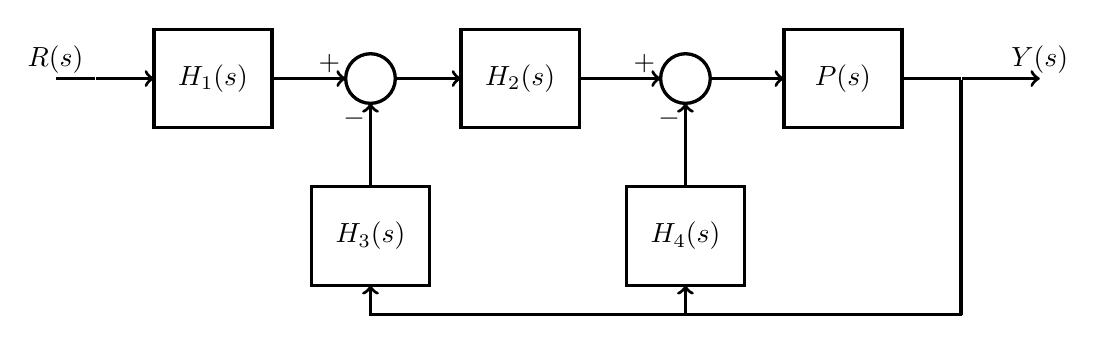
\begin{tikzpicture}[scale=1,inner sep=0pt,outer sep=0pt,very thick,
sysblock/.style={draw,rectangle,inner sep=2pt,minimum width=1.5cm,minimum height=1.25cm,very thick}]

%%% Blocks and Sums for center line %%%%%
\draw (2,0) node[sysblock] (H2) {$H_{1}(s)$};
\draw (4,0) node[draw,circle] (sum1) {$\rule{0pt}{18pt}$};
\draw (5.9,0) node[sysblock] (H3) {$H_{2}(s)$};
\draw (8,0) node[draw,circle] (sum2) {$\rule{0pt}{18pt}$};
\draw (10,0) node[sysblock] (P) {$P(s)$};

	%%% Above center line
	%\draw (4,2) node[sysblock] (H1) {$H_{1}(s)$};
	%%% Below center line
	\draw (4,-2) node[sysblock] (H4) {$H_{3}(s)$};
	\draw (8,-2) node[sysblock] (H5) {$H_{4}(s)$};
%%%%%%%%%%%%%%%%%%%%%%%%%

%%% Center Line Connections
	%%% Include a midpoint for the reference (r)
	\draw[-] (0,0) node[above=2pt] {$R(s)$} -- ++(.5,0) node (r){$$};
	\draw[->] (r) -- (H2.180);

\draw[->] (H2.0) --  (sum1.180) node[above left=2pt] {$+$};
\draw[->] (sum1) -- (H3.180);
\draw[->] (H3.0) -- (sum2.180) node[above left=2pt] {$+$};
\draw[->] (sum2.0) --  (P);

	%%% Include a midpoint for the output (y)
	\draw[-] (P) -- ++(1.5,0) node (y){$$};
	\draw[->] (y) -- ++(1,0) node[above=2pt] {$Y(s)$};

%%% Above center line connections
%\draw[->] (r.0) |-  (H1);
%\draw[->] (H1.0) -| (sum2) node[above right =7pt] {$+$};

%%% Below center line connections
	%%% Include point at the right angle (y2)
	\draw[-] (y) -- ++(0,-3) node (y2){$$}; 
\draw[->] (y2.0) -| (H5.270);
\draw[->] (y2.0) -|  (H4.270);
\draw[->] (H4.90) -- (sum1.270) node[below left=2pt] {$-$};
\draw[->] (H5.90) -- (sum2.270) node[below left=2pt] {$-$};

\end{tikzpicture}

\end{center}
